\section{答案与解析：结构力学基础与技巧班第1次作业答案（几何组成分析）}
\begin{analysisbox}
先算自由度，再按二元体、两刚片、三刚片和瞬变判据复核。判断顺序建议为：先找可并入大地的刚片，再检查约束方向是否共线、平行或交于一点，最后判定有无多余约束。
\end{analysisbox}
\subsection*{第 1 页转写}
1-1、D

解析：采用两刚片规则分析，由于4根链杆平行且不等长，因此为瞬变体系，有

两个多余约束。

1-2、B

解析：原体系的计算自由度

3 3 1 2

4

3

W =\textbackslash{}times -\textbackslash{}times -

=

，故需要再补充三个约束。当

在A处加入固定端时，刚片ABC先并入大地，随后刚片DE与大地由链杆BD和铰

E连接，满足两刚片规则可并入大地，同理FG与大地同样满足两刚片规则，此时

原体系变为无多余约束的几何不变体系。

1-3、C

解析：刚片ABC与大地由三根不共线且不交于一点的链杆A、BD和CE，满足两

刚片规则，原体系为无多余约束的几何不变体系。

1-4、几何常变；1

解析：采用两刚片规则分析，刚片ABCD和有一个多余约束的刚片EFGH仅由两

根链杆CE和DF连接，不满足两刚片规则，原体系为有一个多余约束的几何常变

体系。
\begin{figure}[H]\centering
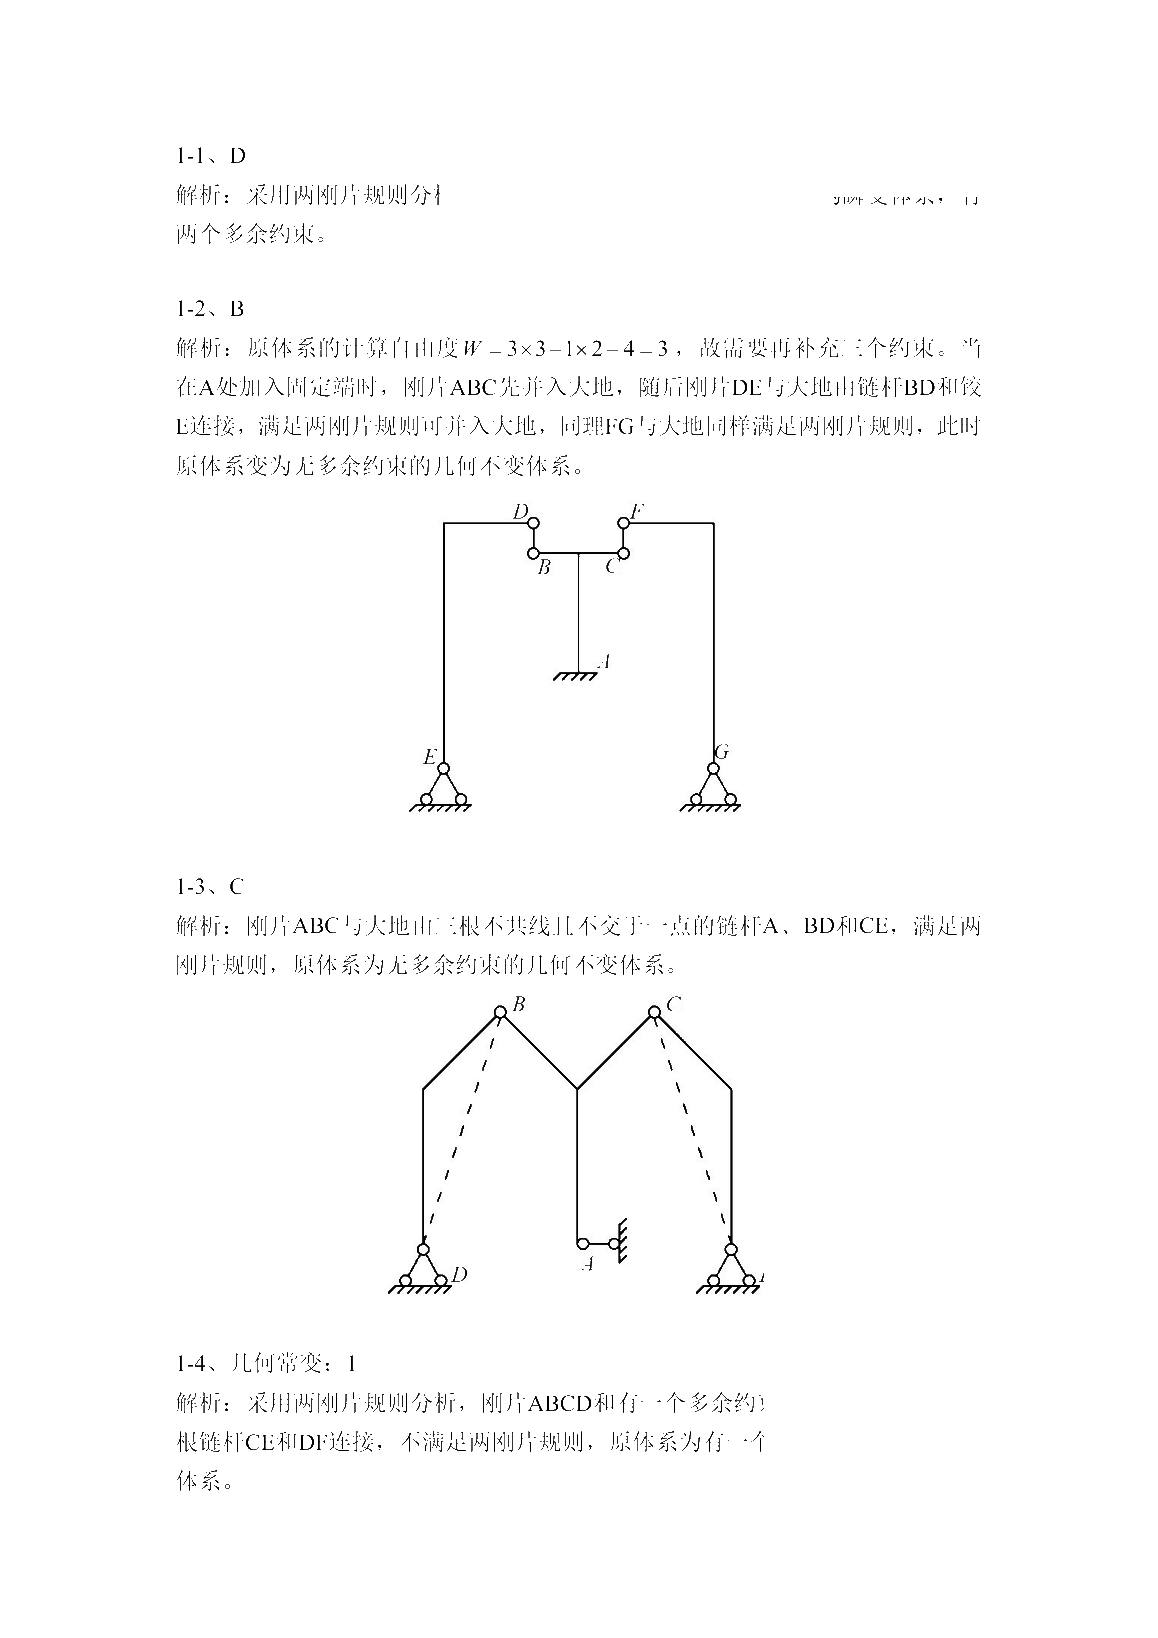
\includegraphics[width=0.92\textwidth]{figures/src01_p001.jpg}
\caption{结构力学基础与技巧班第1次作业答案（几何组成分析） 第 1 页清理图形页}
\end{figure}
\subsection*{第 2 页转写}
1-5、-4

解析：刚片如图所示，计算自由度

5 3

6 2 1 3

4

4

W =\textbackslash{}times -\textbackslash{}times

-\textbackslash{}times -

=-。

1-6、$\times$

解析：由大地依次增加二元体AB、ACB、ADC、DEC、DFE、EGH、EIG、FJI、

FKJ、KLF、KML，原体系为无多余约束的几何不变体系。

1-7、解析：刚片AD、BE可直接并入大地，链杆DE为一个多余约束。随后刚片

EFC与大地由固定端C和铰E连接，满足两刚片规则且有两个多余约束，故原体

系为有3个多余约束的几何不变体系。
\begin{figure}[H]\centering
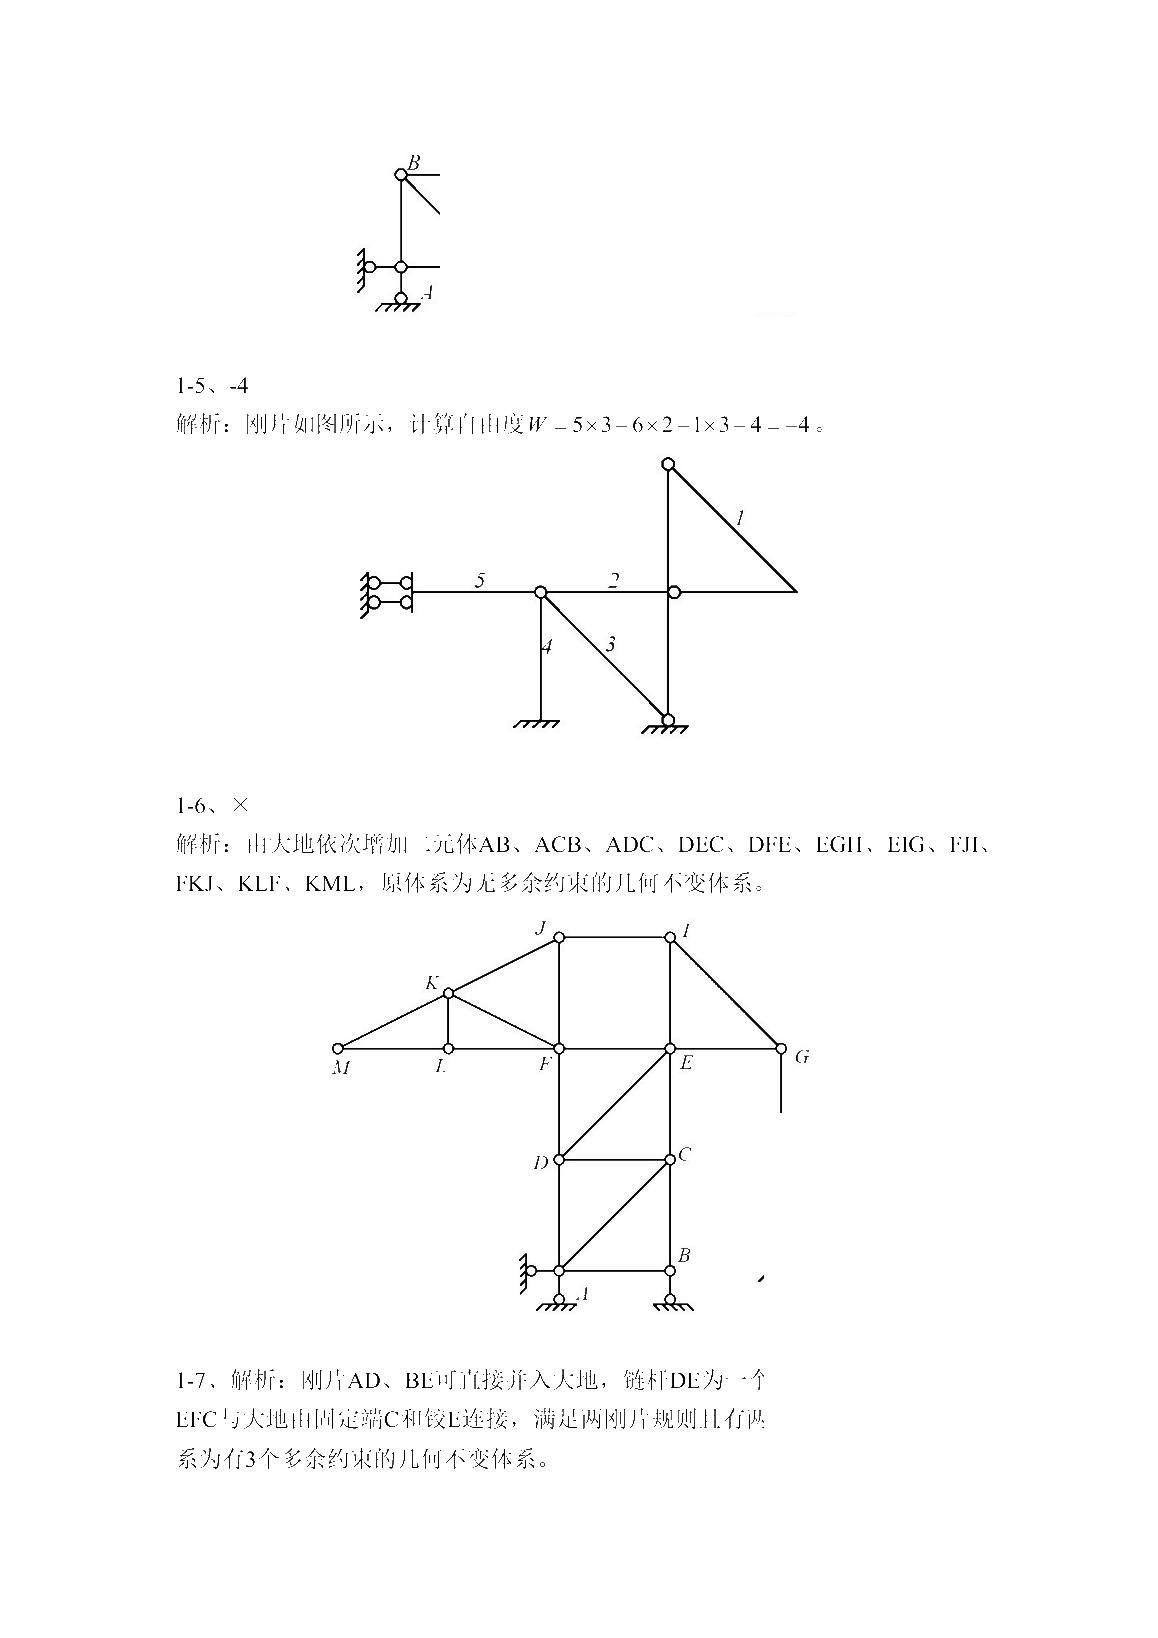
\includegraphics[width=0.92\textwidth]{figures/src01_p002.jpg}
\caption{结构力学基础与技巧班第1次作业答案（几何组成分析） 第 2 页清理图形页}
\end{figure}
\subsection*{第 3 页转写}
1-8、解析：采用三刚片规则分析，各刚片如图所示，刚片ABC与刚片CDE交于

铰C，刚片ABC与刚片GF由链杆BF、AG连接交于铰

2

O ，刚片CDE与刚片FG由

链杆DF、GE连接交于铰

1

O ，三铰不共线满足三刚片规则组成大刚片，后与大地

由三根不共线且不交于一点的链杆支座连接，满足两刚片规则，原体系为无多余

约束的几何不变体系。

1-9、解析：采用三刚片规则分析，各刚片如图所示，刚片ABC与刚片DEF由链

杆BD、CF连接交于无穷远铰

1

O ，刚片ABC与大地刚片由链杆A、CG连接交于铰

A，刚片DEF与大地刚片由链杆FG、E连接交于铰E，三铰共线不满足三刚片规

则，原体系为有一个多余约束的几何瞬变体系。

1-10、解析：计算自由度

12 2

25

1

W =

\textbackslash{}times -

=-。采用两刚片规则分析，刚片ABCD

与刚片DEFB由铰B和铰D共四个约束连接，满足两刚片规则且有一个多余约束，

原体系为有一个多余约束的几何不变体系。
\begin{figure}[H]\centering
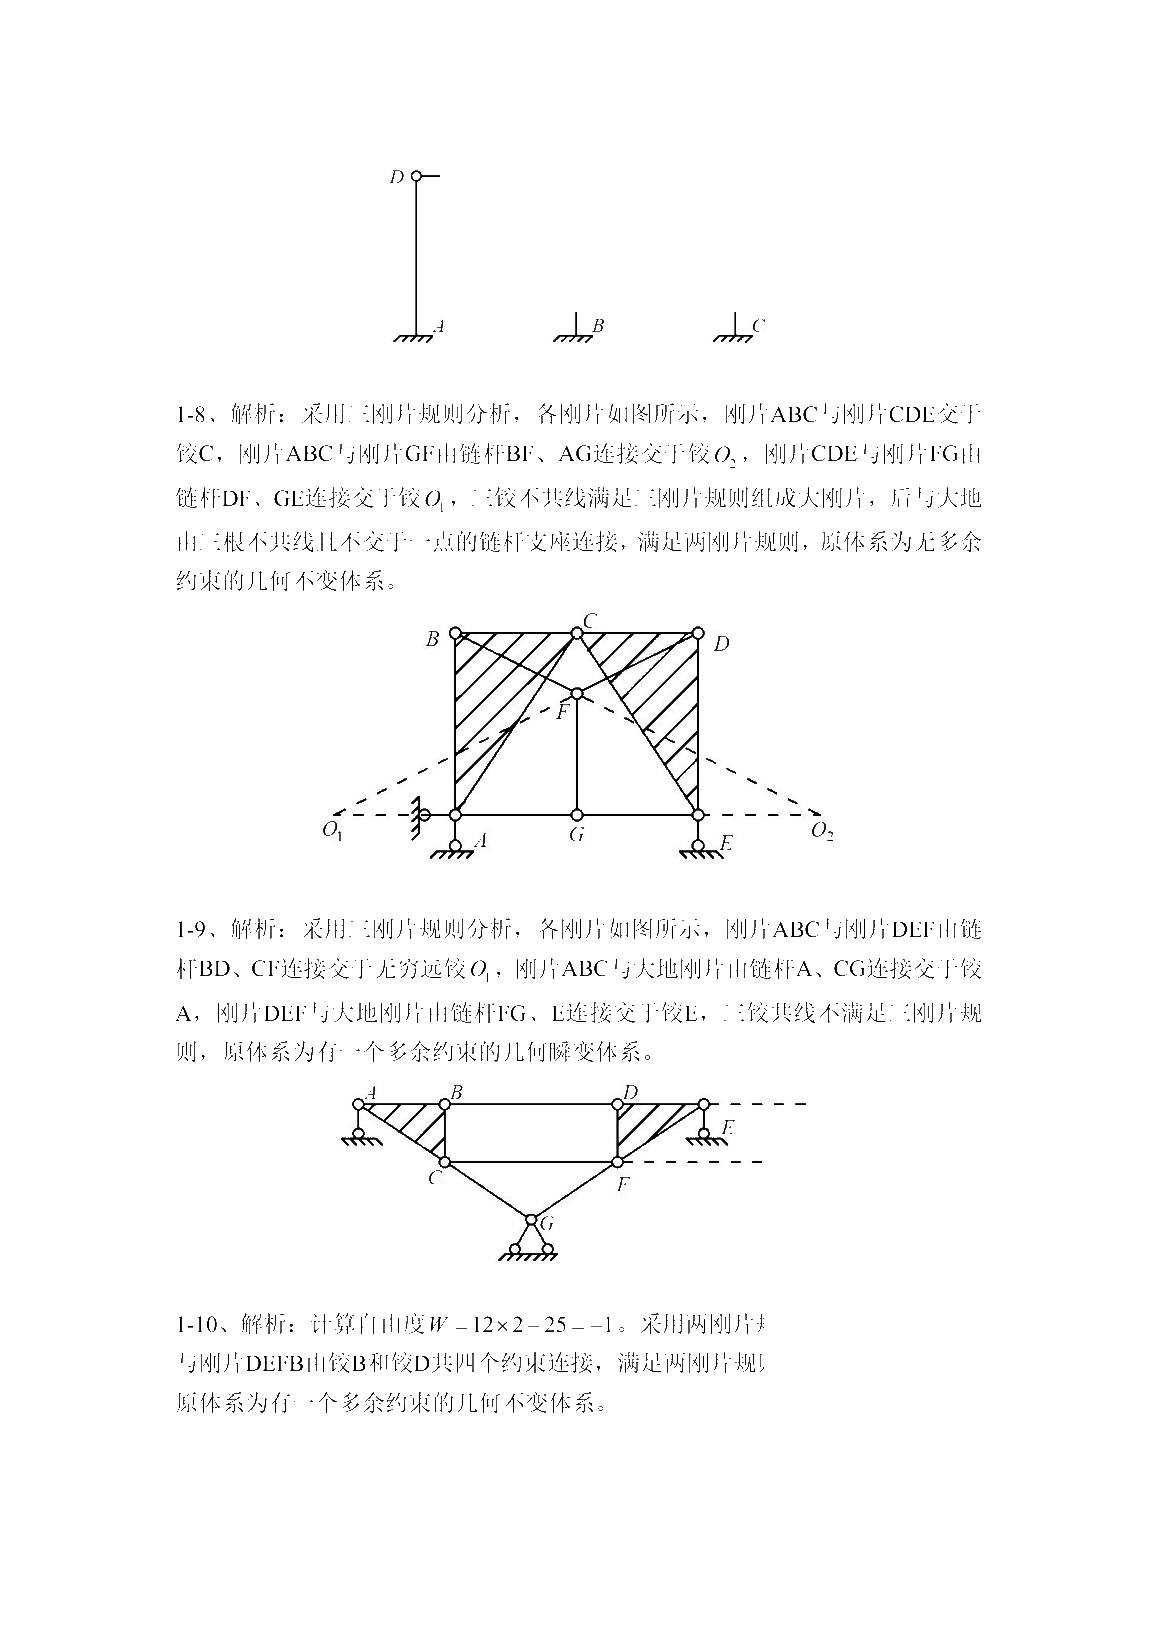
\includegraphics[width=0.92\textwidth]{figures/src01_p003.jpg}
\caption{结构力学基础与技巧班第1次作业答案（几何组成分析） 第 3 页清理图形页}
\end{figure}
\subsection*{第 4 页转写}
1-11、解析：先去掉二元体AB、CEG，随后有两个多余约束的刚片BCD与大地

由三根不共线且不交于一点的链杆D、CF和CG连接，满足两刚片规则，原体系

为有两个多余约束的几何不变体系，两次超静定。

1-12、解析：刚片ABC与大地由三根不共线且不交于一点的链杆支座A和链杆CD

连接，满足两刚片规则可并入大地，随后刚片FBE与大地同样由铰B和链杆F连接

满足两刚片规则，杆GE为多余约束。原体系为有一个多余约束的几何不变体系。

1-13、解析：可将刚片3456等价为链杆34，如图所示。随后采用两刚片规则分析，

刚片14与大地由三根不共线且不交于一点的链杆连接，满足两刚片规则，原体系

为无多余约束的几何不变体系。
\begin{figure}[H]\centering
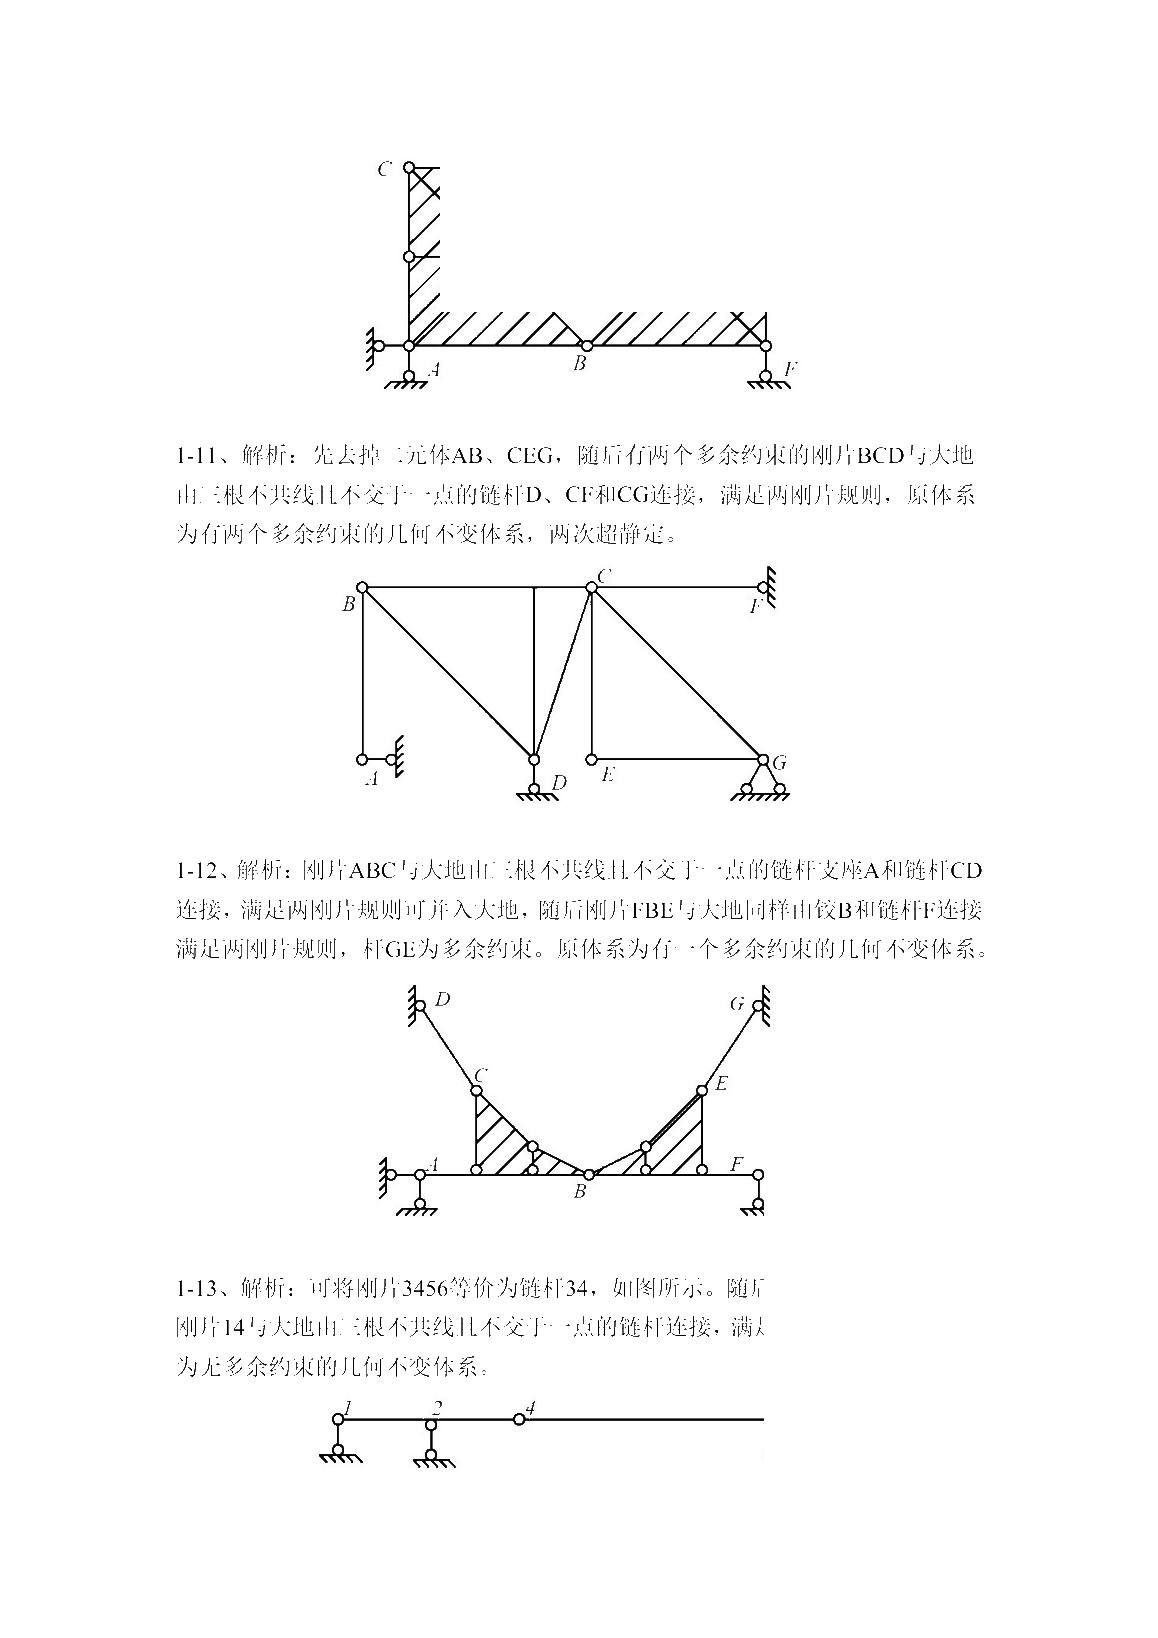
\includegraphics[width=0.92\textwidth]{figures/src01_p004.jpg}
\caption{结构力学基础与技巧班第1次作业答案（几何组成分析） 第 4 页清理图形页}
\end{figure}
\subsection*{第 5 页转写}
1-14、解析：先去掉二元体ABC、AJ、DEF和GFH，随后刚片JCDI与大地由三根

不共线且不交于一点的链杆支座连接，满足两刚片规则，原体系为无多余约束的

几何不变体系。

1-15、解析：计算自由度

7 2 13 1

1

W =

\textbackslash{}times -

\textbackslash{}times =。采用两刚片规则分析，刚片ABC

与刚片DEF仅由链杆CD、BE连接，不满足两刚片规则，原体系为无多余约束的

几何常变体系。

1-16、解析：先去掉二元体ABC，随后采用三刚片规则分析，各刚片如图所示，

刚片ADE与大地刚片由链杆D、EH连接交于无穷远铰

1

O ，刚片CFG与大地刚片

由链杆F、GH连接交于铰

2

O ，刚片ADE与刚片CFG由链杆AC、EG连接交于无穷

远铰

3

O ，三铰共线不满足三刚片规则，原体系为有一个多余约束的几何瞬变体

系。
\begin{figure}[H]\centering
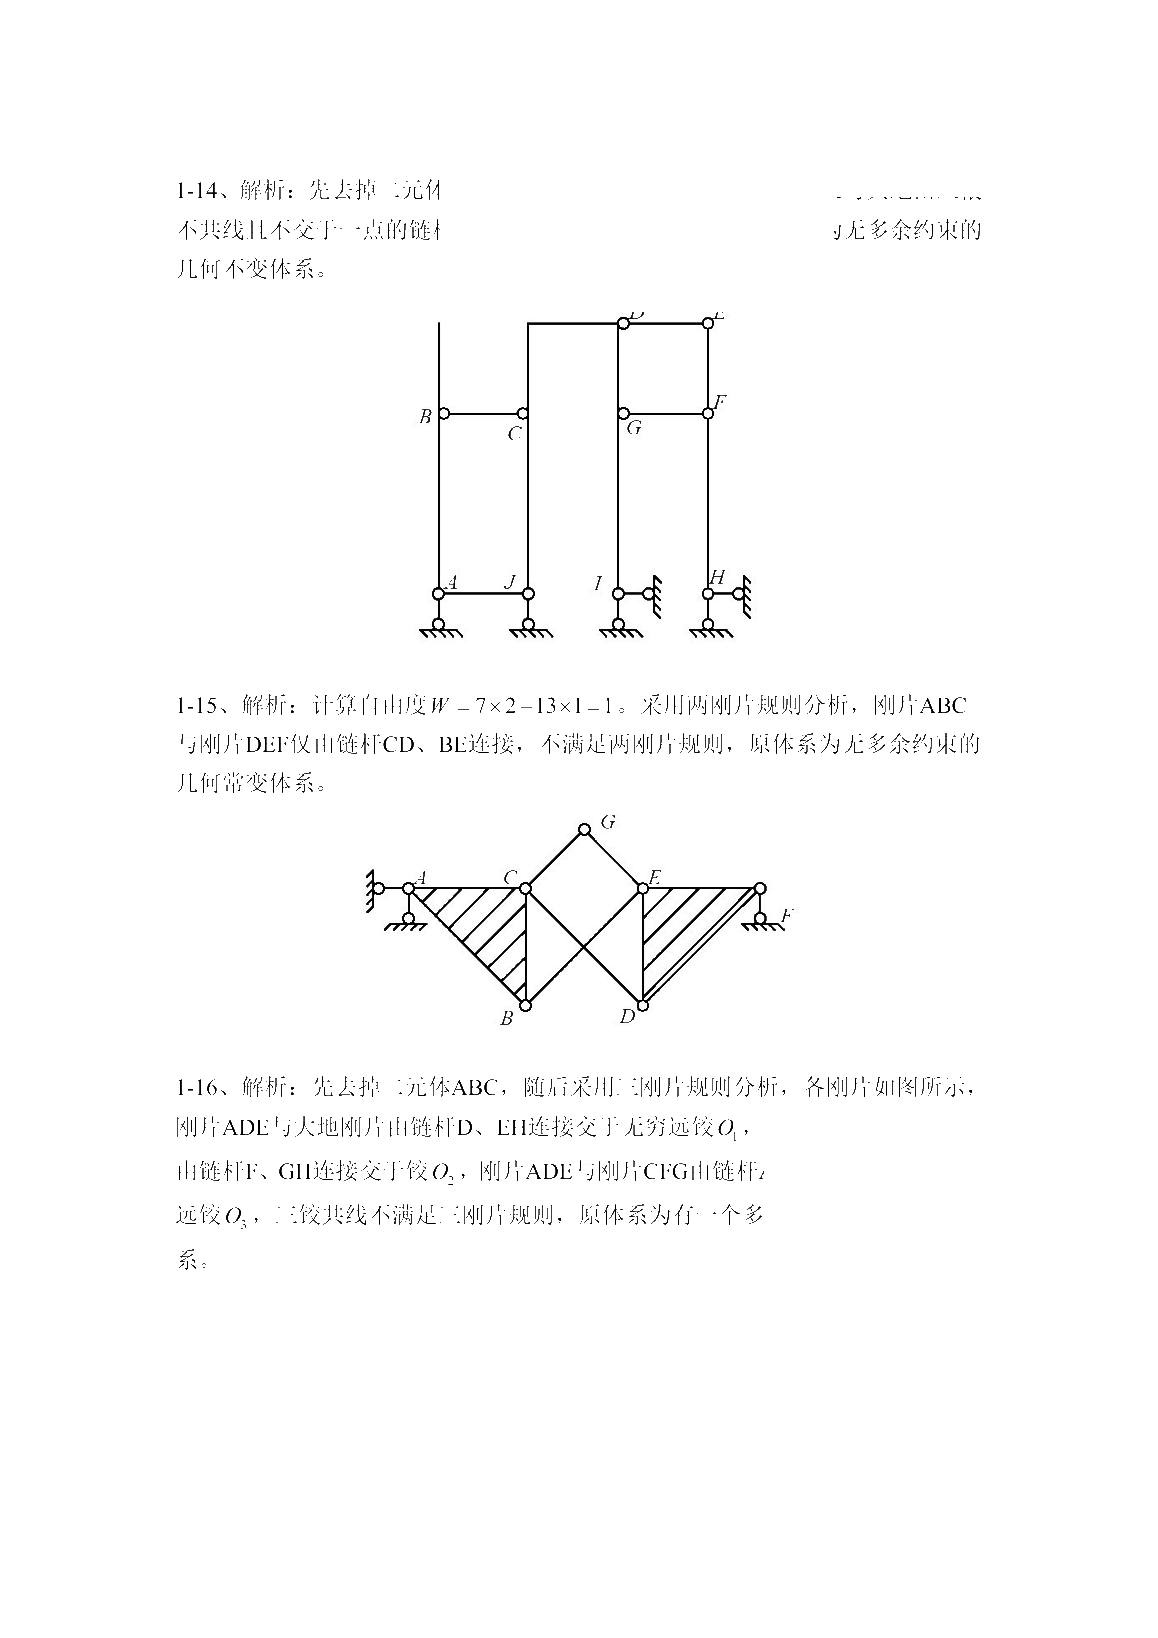
\includegraphics[width=0.92\textwidth]{figures/src01_p005.jpg}
\caption{结构力学基础与技巧班第1次作业答案（几何组成分析） 第 5 页清理图形页}
\end{figure}
\subsection*{第 6 页转写}
1-17、解析：计算自由度

4 3

3 2

7 1

1

W =

\textbackslash{}times -\textbackslash{}times

-\textbackslash{}times =-。刚片AB可先并入大地，随

后采用两刚片规则分析，杆CD与大地由三根不共线且不交于一点的链杆BC和支

座D连接，满足两刚片规则，CE杆为多余约束，故原体系为有一个多余约束的几

何不变体系。
\begin{figure}[H]\centering
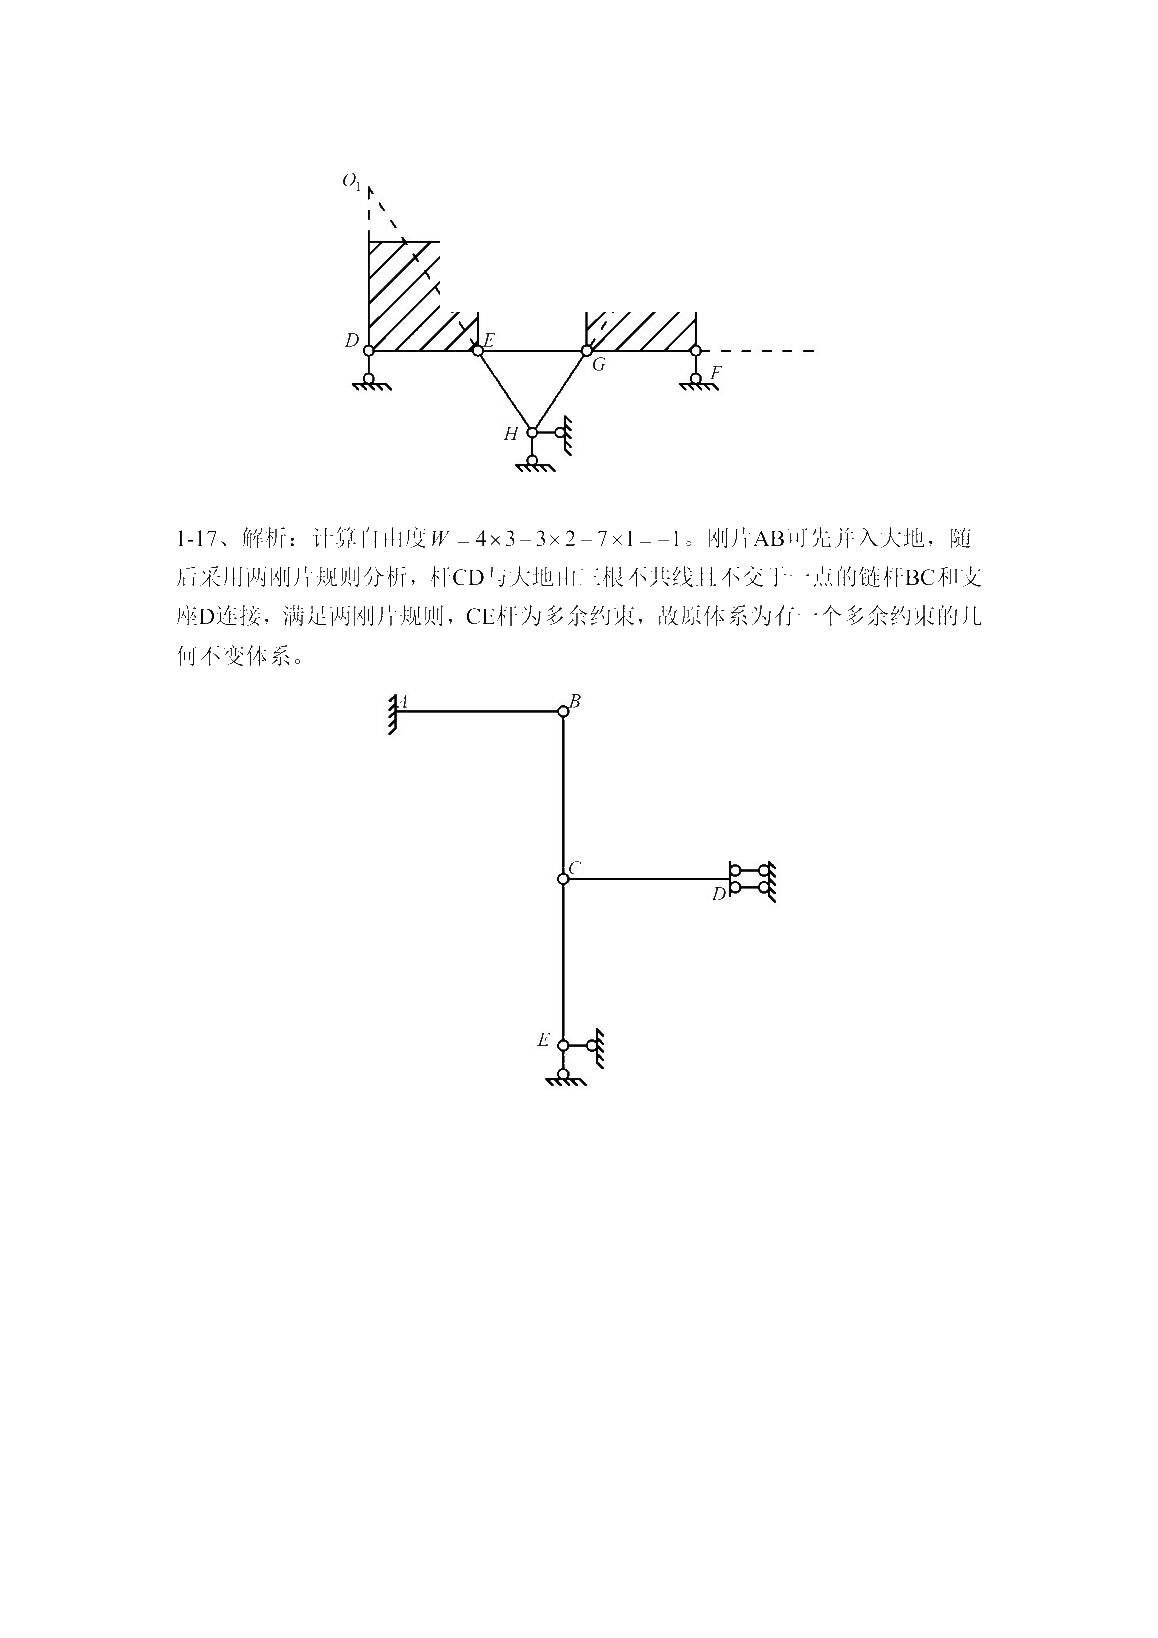
\includegraphics[width=0.92\textwidth]{figures/src01_p006.jpg}
\caption{结构力学基础与技巧班第1次作业答案（几何组成分析） 第 6 页清理图形页}
\end{figure}
